\documentclass{tufte-handout}

\title{Section 2.4 Average Rate of Change}

\author[AW]{Ammon Washburn}

\usepackage{graphicx} % allow embedded images
  \setkeys{Gin}{width=\linewidth,totalheight=\textheight,keepaspectratio}
  \graphicspath{{graphics/}} % set of paths to search for images
\usepackage{amsmath}  % extended mathematics
\usepackage{booktabs} % book-quality tables
\usepackage{units}    % non-stacked fractions and better unit spacing
\usepackage{multicol} % multiple column layout facilities
\usepackage{lipsum}   % filler text
\usepackage{fancyvrb} % extended verbatim environments
  \fvset{fontsize=\normalsize}% default font size for fancy-verbatim environments

% Standardize command font styles and environments
\newcommand{\doccmd}[1]{\texttt{\textbackslash#1}}% command name -- adds backslash automatically
\newcommand{\docopt}[1]{\ensuremath{\langle}\textrm{\textit{#1}}\ensuremath{\rangle}}% optional command argument
\newcommand{\docarg}[1]{\textrm{\textit{#1}}}% (required) command argument
\newcommand{\docenv}[1]{\textsf{#1}}% environment name
\newcommand{\docpkg}[1]{\texttt{#1}}% package name
\newcommand{\doccls}[1]{\texttt{#1}}% document class name
\newcommand{\docclsopt}[1]{\texttt{#1}}% document class option name
\newenvironment{docspec}{\begin{quote}\noindent}{\end{quote}}% command specification environment

\newtheorem{mydef}{Definition}
\providecommand{\floor}[1]{\left \lfloor #1 \right \rfloor }

\begin{document}
\maketitle

\begin{abstract}
Learn how to find and use secant lines in functions
\end{abstract}
\section{ARC}
This is similar to the idea of average speed or the slope of lines but applied to lots of functions.

\begin{mydef}
The average rate of change or ARC of a function f(x) between $x=a$ and $x=b$ is $\frac{change in f}{change in x} = \frac{f(b)-f(a)}{b-a}$
\end{mydef}

This is the slope of the secant line that passes through (a,f(a)) and (b,f(b)).  Find the ARC of $y(x) = x^2+2x$ on the following intervals: 

a) $-5 \leq x \leq -1$ \hspace{1 cm} b) $-3 \leq x \leq 3 $ \hspace{1 cm} c) $a \leq x \leq a + h$

Answers: a) -4 \hspace{1 cm} b) 2 \hspace{1 cm} c) 2a + 2 +h

Example:
\begin{figure}
\centering
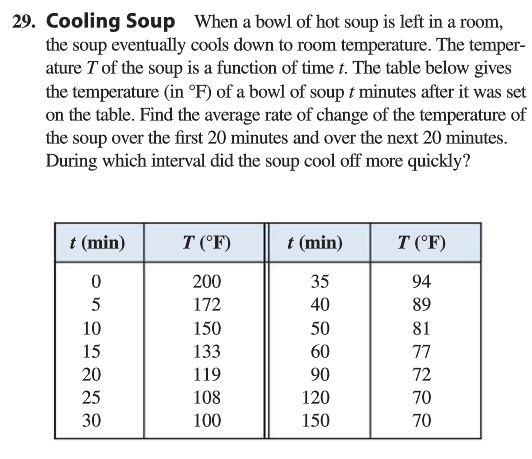
\includegraphics[width = \linewidth]{2-4CoolingProblem.png}
\end{figure}

a) First 20 minutes the ARC is -4.05 degrees F per minute 

b) Next 20 minutes the ARC is -1/5 degrees F per minute
\section{Quiz}
By each interval, it could mean any interval but here is a hint.  If the ARC of one interval is a and the ARC of another interval is b then the ARC over the interval is somewhere between a and b.  In other words the fastest one will be over the shortest intervals.










\end{document}
